% !TeX program = xelatex
\documentclass[a4paper,12pt]{article}
\usepackage[left=2.0cm, right=2.0cm, top=2.5cm, bottom=2.0cm]{geometry}
\usepackage{indentfirst}
\usepackage{amsmath, amssymb, amsfonts}
\usepackage{multirow}
\usepackage{graphicx}
\usepackage{xeCJK}
\usepackage{fancyhdr}
\usepackage{verbatim}
\usepackage{algorithm}
\usepackage{algpseudocode}
\usepackage{hyperref}
\pagestyle{fancy}
\lhead{}
\chead{图形学大作业系统报告}
\rhead{陈劭源(161240004)}
\lfoot{}
\cfoot{}
\rfoot{\thepage}
\setCJKmainfont[BoldFont=SimHei,ItalicFont=KaiTi]{SimSun}
\setCJKmonofont{KaiTi}
\setmainfont{Times New Roman}
\setmonofont{Courier New}
\renewcommand\refname{参考文献}
\graphicspath{{figures/}}

\title{图形学大作业系统报告}
\author{陈劭源(161240004) \\ \href{mailto:sy\_chen@smail.nju.edu.cn}{sy\_chen@smail.nju.edu.cn}}
\date{\today}

\begin{document}
\maketitle

\section{综述}



\section{算法介绍}
绘制曲线$f(x,y) = 0$的基本原则是:当$\left|\frac{\mathrm{d}y}{\mathrm{d}x} \big|_{(x_0, y_0)} \right| \leq 1$时,沿$x$轴递进采样画点;当$\left|\frac{\mathrm{d}y}{\mathrm{d}x} \big|_{(x_0, y_0)} \right| > 1$时,沿$y$轴递进采样画点。这样可以保证相邻两个绘制点$(x_i, y_i), (x_{i+1}, y_{i+1})$之间满足$\max\{|x_i - x_{i+1}|, |y_i - y_{i+1}|\} = 1$。

\subsection{DDA算法}

DDA算法是利用对曲线微分方程积分的方法来绘制曲线的。DDA算法通常用于绘制线段、多边形等,但也可用来绘制非线性曲线\cite{wiki:DDA}。对于直线$y = kx + b$ $(|k| \leq 1)$,DDA算法在每次递增$x$时,对$y$增加$k$,并将取整后的值作为当前绘制点。利用DDA算法绘制线段的伪代码如下:

\begin{algorithm}[htb] 
\caption{DDA画线算法} 
\label{alg:DDA} 
\begin{algorithmic}[1] 
\Require 
线段的两个端点$(x_1, y_1)$, $(x_2, y_2)$。假定$x_1 < x_2, |x_2 - x_1| \geq |y_2 - y_1|$。
\State $y = y_1, k = \frac{y_2 - y_1}{x_2 - x_1}$
\For{$x = x_1$ to $x_2$}
    \State 绘制点 $([x], [y])$
    \State $y = y + k$
\EndFor
\end{algorithmic} 
\end{algorithm}

\subsection{Bresenham算法}

Bresenham算法的基本思想是,通过判断下两个绘制点的中点在直线的哪一侧来决定选取哪一个决策点。判断中点在直线哪一侧可以通过维护一个决策变量$\Delta$来实现,而决策变量的维护通常可以利用整数的加减法实现\cite{wiki:Bresenham},因此Bresenham算法比DDA算法更加高效。

对于以$(x_1, y_1), (x_2, y_2)$ (假设$x_1 < x_2, y_1 \leq y_2, |x_1 - x_2| \geq |y_1 - y_2|$)为端点的线段,它的直线方程为

$$ (y - y_1) (x_2 - x_1) = (y_2 - y_1)(x - x_1) $$

故可取决策变量$\Delta(x, y) = 2[(y_2 - y_1)(x - x_1) - (y - y_1)(x_2 - x_1)]$,并根据$\Delta(x_i+1, y_i+0.5)$的符号决定绘制点。当决策变量为正时,递增$y$,否则不递增$y$。决策变量可用以下方式维护:

$$ \Delta(x_i+1, y_i+0.5) = \Delta(x_i, y_i) + 2\Delta y - \Delta x $$
$$ \Delta(x_i+1, y_i+1) = \Delta(x_i+1, y_i+0.5) - \Delta x $$
$$ \Delta(x_i+1, y_i) = \Delta(x_i+1, y_i+0.5) + \Delta x $$

Bresenham算法的伪代码如下

\begin{algorithm}[htb] 
\caption{Bresenham画线算法} 
\label{alg:DDA} 
\begin{algorithmic}[1] 
\Require 
线段的两个端点$(x_1, y_1)$, $(x_2, y_2)$。假定$x_1 < x_2, y_1 \leq y_2, |x_2 - x_1| \geq |y_2 - y_1|$。
\State $y = y_1, \Delta x = x_2 - x_1, \Delta y = y_2 - y_1$
\State $\Delta = -\Delta x$
\For{$x = x_1$ to $x_2$}
	\If{$\Delta \geq 0$}
	\State $y = y + 1, \Delta = \Delta - \Delta x$ 
	\Else
	\State $\Delta = \Delta + \Delta x$
	\EndIf
    \State 绘制点 $(x, y)$
    \State $\Delta = \Delta + 2\Delta y - \Delta x$
\EndFor
\end{algorithmic} 
\end{algorithm}

\subsection{\dots}
\dots
		
\section{系统介绍}
\begin{figure}
\centering
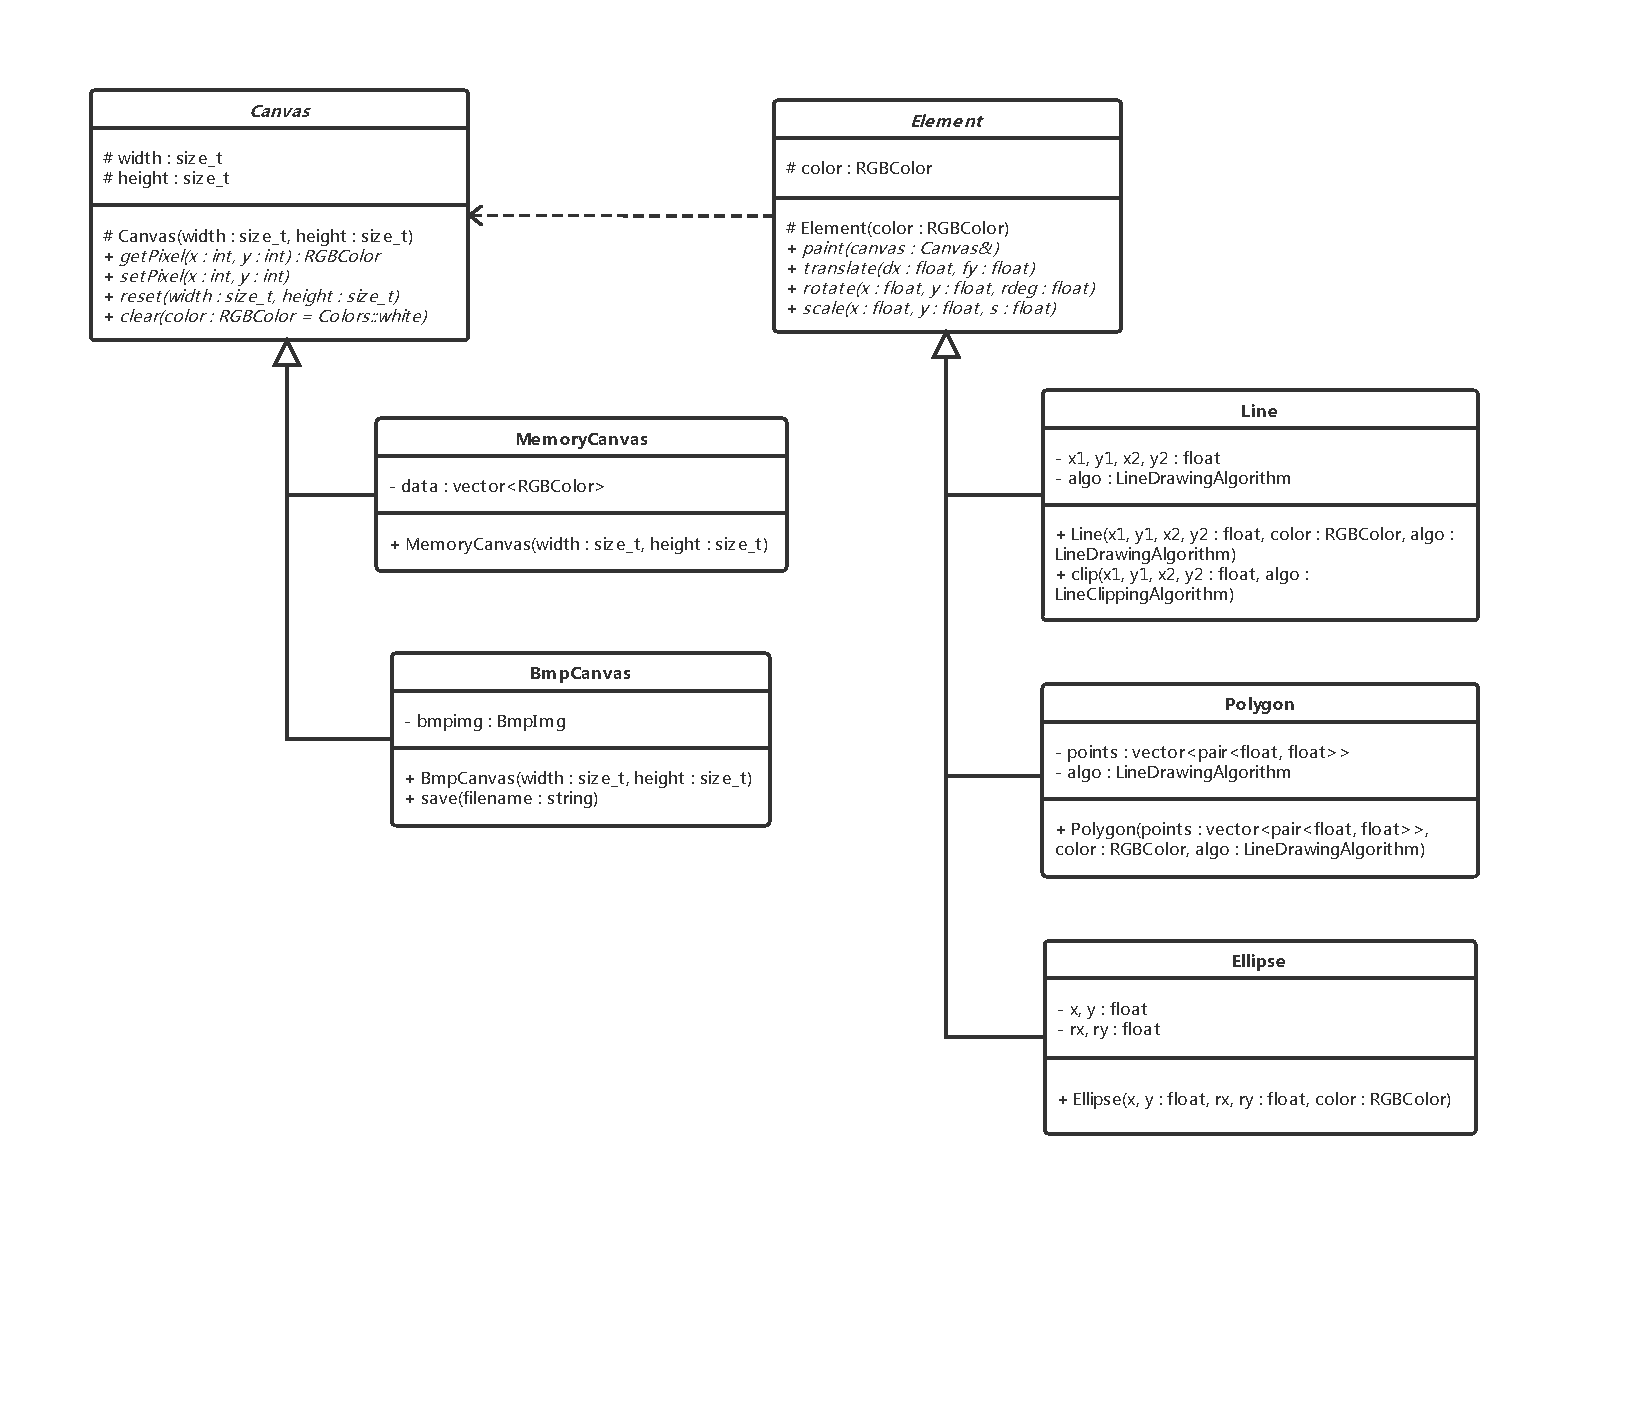
\includegraphics[width=\linewidth]{uml.pdf}
\caption{系统的UML类图}
\end{figure}
\section{总结}
\dots

\bibliographystyle{unsrt}%
%"xxx" should be your citing file's name.
\bibliography{report}
\end{document}
